La nouvelle méthode de traitement des homographies repose sur la décomposition d'une homographie qui permet d'interpréter cette dernière en terme de mouvement de caméra. La partie ci-dessous présente cette décomposition.

\ssse{Modélisation de mouvement de caméra}
\label{mouv_de_camera}
On étudie ici un cas a priori particulier d'homographie $h$ : les homographies que l'on peut interpréter comme un mouvement de caméra idéale. On montrera par la suite que c'est en fait un cas général.

Nous modéliserons la situation en supposant que la scène filmée est plane. Cela suppose que l'on filme une surface soit sans aucun relief, soit avec un relief négligeable devant la distance à la caméra, afin qu'il ne soit pas perceptible. La figure \ref{shmdecomp} illustre la modélisation utilisée pour la caméra idéale, les paramètres introduits sur ce schéma seront définis dans les définitions et notations \ref{defpoint}. La caméra idéale se modélise donc par la projection d'un plan sur un autre en passant par un foyer $F$, en négligeant les lentilles ou les dispositifs correcteurs présents dans les caméras réelles.

\begin{figure}[h!]

\centering
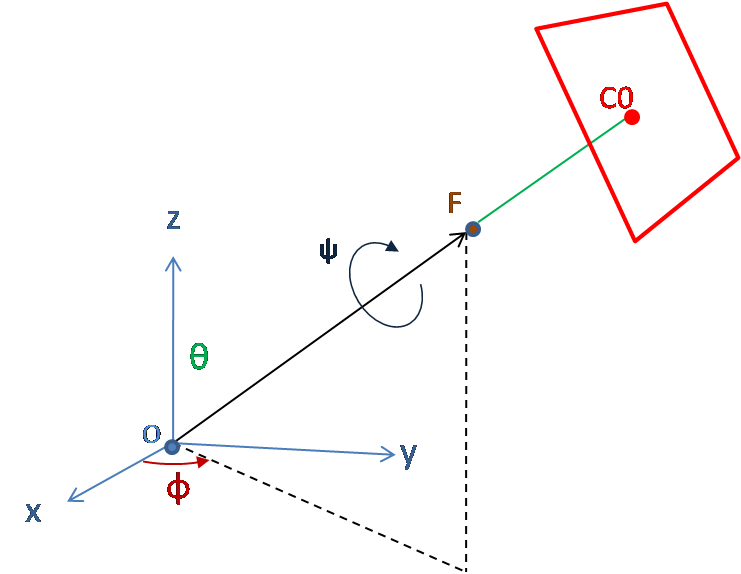
\includegraphics[width=10cm]{shema_decomp.png}
\caption{Illustration d'un mouvement de caméra $(X_v =0)$ (les translations ont été omises pour plus de clarté. $F$ représente le point focal de la caméra, le plan rouge est le plan image de la caméra. Un point du plan image est le projeté passant par $F$ d'un point du plan $(x,y)$. (cf. partie \ref{mouv_de_camera})}
\label{shmdecomp}
\end{figure}


On se place dans l'espace vectoriel $\mathbb{R}^{3}$ on note $O$ l'origine $(0,0,0)$ et $(\xbf_0,\ybf_0,\zbf_0)$ la base canonique.
\begin{itemize}
\item Soient $F$ et $C_0$ deux points distincts de  $\mathbb{R}^{3}$.
\item Soit $\mathcal{P}$ le plan affine passant par $C_0$ de vecteur normal $\overrightarrow{FC_0}$.
\item On note $\wbf$ le vecteur $\frac{\overrightarrow{FC_0}}{|| \overrightarrow{FC_0}||}$
\item On note $\delta$ la distance  $|| \overrightarrow{FC_0}||$
\end{itemize}
\begin{Def}
L'application projective $H$, est l'application qui à un point $X$ de $\mathbb{R}^{3}$ associe le point d'intersection entre la droite $(XF)$ et le plan $\mathcal{P}$. $H$ dépend du triplet $(F,\wbf,\delta)$.
\end{Def}
\begin{remarques}
\begin{itemize}
\item $F$ est la position de l'objectif de la caméra et le plan $\mathcal{P}$ est l'écran de la caméra sur lequel est projetée l'image. L'axe optique de la caméra est la droite $(FC_0)$ de vecteur directeur $\wbf$, $\delta$ est la distance entre l'objectif et l'écran.
\item A un point de $\mathbb{R}^3$  l'application $H$ associe le  point de $\mathcal{P}$ correspondant à son image a travers la caméra.
\end{itemize}
\end{remarques}
Soit $\mathcal{P}'$ le plan affine de $\mathbb{R}^{3}$ passant par $F$ et parallèle au plan $\mathcal{P}$.
\begin{lem}
$H$ est définit sur $\mathbb{R}^3 \setminus \mathcal{P}'$ et on a  
\begin{equation}
H(X) = C_0 +  \delta \frac{\overrightarrow{XF}-(\overrightarrow{XF}\cdot \wbf )\wbf}{\wbf \cdot \overrightarrow{XF}} 
\label{formul_lem_app_proj}
\end{equation}
\label{lem_app_proj}
\end{lem}
\begin{proof}
Si $X\in \mathbb{R}^3 \setminus \{F\}$ la droite $(XF)$ et admet un point d'intersection avec $\mathcal{P}$ si et seulement elle n'est pas parallèle à $\mathcal{P}$ donc si et seulement si $X\in \mathbb{R}^3 \setminus \mathcal{P}'$. Dans ce cas il existe $t_X\in \mathcal{R}$ tel que 
\begin{equation*}
H(X)=X+t_{X}\overrightarrow{XF}.
\end{equation*}
Comme $H(X)\in P_{2}$ alors
\begin{equation*}
\overrightarrow{FH(X)}\cdot \wbf =\delta.
\end{equation*}
En réinjectant l'expression de $H(X)$ on obtient
\begin{equation*}
t_{X}=1+\frac{\delta}{\wbf \cdot \overrightarrow{XF}},
\end{equation*}
 On en déduit que 
\begin{equation*}
H(X) = C_0 +  \delta \frac{\overrightarrow{XF}-(\overrightarrow{XF}\cdot \wbf )\wbf}{\wbf \cdot \overrightarrow{XF}}.
\end{equation*}
\end{proof}
\begin{remarque}
Le plan $\mathcal{P}'$ correspond à un angle mort de la caméra, dans le cas d'une caméra réelle cet angle mort devrait occuper au moins un demi espace 
\end{remarque}
On note $P$ le plan $(O,\xbf_0,\ybf_0)$.
\begin{Def} On appelle point visé le point d'intersection entre la droite $(FC_0)$ et le plan $P$ lorsqu'il existe. Le point visé existe si et seulement si $(FC_0)$ n'est pas parallèle à  $\mathcal{P}$. Lorsqu'il existe on le note $X_v$ et on a
\begin{equation*}
X_v=F-\wbf \delta'~~~~~~\delta'=\frac{\overrightarrow{OF}\cdot \zbf_0}{\wbf \cdot \zbf_0}
\label{formule_point_vise}
\end{equation*}
\label{point_vise}
\end{Def}
\begin{remarque}
Le point visé est le point de $P$ visé par la caméra, les mouvements de la caméra se font autour de ce point. Il est possible qu'une caméra n'ait pas de point visé dans se cas il est situé à l'infini, la caméra vise l'horizon. 
\end{remarque}
On suppose dans la suite que le point visé existe.
\begin{Def}
L'application projective planaire $H^*$ associée à $H$ est la restriction de $H$ à $P\setminus (\mathcal{P}'\cap P)$ 
Si $\wbf \perp P $ alors $H^*$ est définit sur $P$ sinon $H^*$ est définit sur $P\setminus D$ où $D$ est la droite
\begin{equation*}
D=\left\{ X\in P | \overrightarrow{XF}\cdot \wbf = 0\right\}
\end{equation*}
\end{Def}
\begin{remarque}
\begin{itemize}
\item Si on suppose que la scène filmée est suffisamment plane pour que l'on puisse  négliger tout relief on peut l'assimiler au plan $P$ . Alors à un point $X\in P$  de la scène filmée, l'application $H^*$ associe le point de $P_2$ correspondant à son image à travers la caméra.
\item La droite $D'=\{ X \in \mathcal{P} | \overrightarrow{XF} \cdot \zbf_0 =0 \}$ est appelé l'horizon de $H^*$.
\end{itemize}

\end{remarque}
On peut munir le plan affine $\mathcal{P}$ d'un repère orthonormé direct $(C,\ubf,\vbf)$ 
\begin{Def}
 L'homographie associée à $H^*$ dans le repère $(C,\ubf,\vbf)$ est l'application
\begin{equation}
h : (x,y)  \mapsto \left( \overrightarrow{CH^*(X)}\cdot \ubf , \overrightarrow{CH^*(X)}\cdot \vbf \right)
\label{formule_homographie_H}
\end{equation}


où $X=x~\xbf_0 + y~\ybf_0 $.
\label{def_homographie_H}
\end{Def}
Si on note encore $D,D'$ les droites de $\mathbb{R}^2$ obtenue lorsque $P$ et $\mathcal{P}$ sont munit des repère $(O,\xbf,\ybf)$ et $(C,\ubf,\vbf)$ alors $h:\mathbb{R}^2  \setminus D \mapsto \mathbb{R}^2  \setminus D'$ est une bijection.
\begin{remarque}
A un point $X\in P$ de coordonnées $(x,y)$  l'application $h$ associe les coordonnées  du point $H^*(X)$ dans l'image numérique obtenue après acquisition par la caméra. 
\end{remarque}
L'orientation de la base $(\ubf,\vbf,\wbf)$ par rapport à la base $(\xbf_0,\ybf_0,\zbf_0)$ peut être définie grâce aux trois angles d'Euler $(\phi , \theta ,\psi )$ (figure \ref{image_graph})
\begin{itemize}
\item $\phi$ est la précession autour de l'axe $(X_v ,\zbf_0)$
\item $\theta$ est l'inclinaison par rapport à l'axe $(X_v , \zbf_0 )$
\item $\psi$ est la rotation propre autour de l'axe $(X_v , \wbf )$
\end{itemize}
On note $\cbf= \left (\overrightarrow{C_0 C}\cdot \ubf , \overrightarrow{C_0 C}\cdot \vbf \right)$ et $\xbf_v=\left( \overrightarrow{O X_v}\cdot \ubf , \overrightarrow{O X_v}\cdot \vbf \right )$.\\
\begin{prop}
 L'homographie  $h$ se factorise sous la forme
 
\begin{equation}
h = \tau_{\cbf}   \circ R_{\psi} \circ z_{\frac{\delta}{\delta'}} \circ h_{\theta,\delta'} \circ R_{\phi} \circ \tau_{\xbf_v}
\label{formul_decomp}
\end{equation}
Où $R_{\alpha}$ est la rotation d'angle $\alpha$,$z_\lambda$ est la dilatation de facteur $\lambda$, $\tau_\ybf$ est  la translation du vecteur $-\ybf$ et $h_{\theta,\delta'}$ est l'homographie unidirectionnelle (cf. définition \ref{homo_uni_direc})
\begin{equation}
h_{\theta,\delta'}(x,y)=\left(\frac{-cos(\theta)x}{1-\frac{sin(\theta)}{\delta'}x} ,\frac{-y}{1-\frac{sin(\theta)}{\delta'}x}\right)
\label{mise_perspective}
\end{equation}
\label{prop_decomp}
\end{prop}

\begin{figure}[h!]
\centering
\subfigure[rotation d'angle $\phi$]{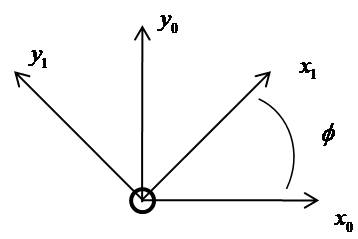
\includegraphics[width=5cm]{graphe1.jpg}}
\subfigure[rotation d'angle $\theta$]{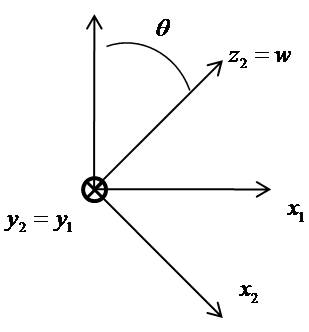
\includegraphics[width=5cm]{graphe2.jpg}}
\caption{(cf partie \ref{figure_de_rotations_18})}
\label{img_angles}
\end{figure}

\begin{figure}[h!]
\centering
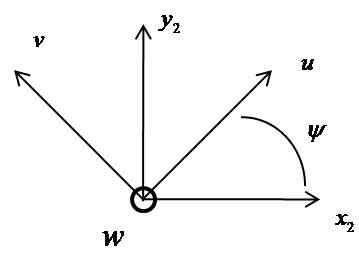
\includegraphics[width=5cm]{graphe3.jpg}
\caption{rotation propre (cf partie \ref{figure_de_rotations_18})}
\label{decompgeo_rotationPropre}
\end{figure}

\begin{proof}
Grâce à la formule (\ref{formule_homographie_H}) de la définition (\ref{def_homographie_H}) et la formule  (\ref{formul_lem_app_proj}) du lemme (\ref{lem_app_proj}) on obtient
\begin{equation*}
h((x,y))=\left( \delta \frac{\overrightarrow{XF}\cdot \ubf}{\overrightarrow{XF} \cdot \wbf} +\overrightarrow{CC_0 } \cdot \ubf, \delta \frac{\overrightarrow{XF}\cdot \vbf}{\overrightarrow{XF} \cdot  \wbf}+\overrightarrow{CC_0 }\cdot \vbf \right)
\end{equation*}
où $X=x \xbf_0 + y \ybf_0 $.\\
En introduisant le point visé $X_v$ (définition \ref{point_vise} formule \ref{formule_point_vise}) et la translation $\tau_c$ on obtient 
\begin{equation}
(\tau_\cbf^{-1} \circ h)((x,y)) = \left ( -\delta \frac{\overrightarrow{X_vX}\cdot \ubf}{\delta' -\overrightarrow{X_vX} \cdot \wbf},-\delta \frac{\overrightarrow{X_vX}\cdot \vbf}{\delta' -\overrightarrow{X_vX} \cdot \wbf} \right)
\label{decomp_formul_intermediaire_1}
\end{equation}
On peut définir les bases intermédiaires $(\xbf_1 ,\ybf_1 ,\zbf_1)$  $(\xbf_2 ,\ybf_2 ,\zbf_2)$ , afin de décomposer les trois rotations $\phi,\theta,\psi$ (figures \ref{img_angles} et \ref{decompgeo_rotationPropre} ).
On obtient alors les relations
\begin{equation*}
\ubf=\cos(\psi)\xbf_{2}+\sin(\psi)\ybf_{2} , \vbf=-\sin(\psi)\xbf_{2}+\cos(\psi)\ybf_{2} \text{ et } \wbf=\zbf_2.
\end{equation*}
On pose $R_{s}$ la rotation d'angle $s$, on obtient alors grâce à la formule (\ref{decomp_formul_intermediaire_1}) 
\begin{equation*}
(\tau_{\cbf}^{-1} \circ h)((x,y)) = R_{\psi}\left(\frac{\delta \overrightarrow{X_v X}\cdot \xbf_{2} }{\delta'-\zbf_2 \cdot \overrightarrow{X_v X}},\frac{\delta \overrightarrow{X_v X}\cdot \ybf_{2}}{\delta'-\zbf_2 \cdot \overrightarrow{X_v X}}  \right).
\end{equation*}
On pose $i$ l'application définie par $i(x,y)=x \xbf_0 + y \ybf_0$, comme $i(\xbf_v)=\overrightarrow{O X_v}$ on obtient alors 
\begin{equation*}
(R_{\psi}^{-1} \circ \tau_{\cbf}^{-1}  \circ h)((x,y))=\delta \left(\frac{-i(\tau_{\xbf_v} ((x,y)))\cdot \xbf_{2} }{\delta'-\zbf_2 \cdot i(\tau_{\xbf_v} ((x,y)))},\frac{-i(\tau_{\xbf_v} ((x,y)))\cdot \ybf_{2}}{\delta'-\zbf_2 \cdot i(\tau_{\xbf_v} ((x,y)))}  \right) 
\end{equation*}

Comme $\zbf_{2}=cos(\theta)\zbf_{1}+sin(\theta)\xbf_{1}$, $\xbf_{2}=cos(\theta)\xbf_{1}-sin(\theta)\zbf_{1}$ (figure \ref{img_angles}) et $\zbf_{1}\perp P_{1}$, on a

\begin{equation*}
(R_{\psi}^{-1} \circ \tau_{\cbf}^{-1}  \circ h)((x,y))=\frac{\delta}{\delta'}\left(\frac{-\cos(\theta)i(\tau_{\xbf_v} ((x,y)))\cdot \xbf_{1} }{1-\frac{sin(\theta)}{\delta'}\xbf_{1}\cdot i(\tau_{\xbf_v}((x,y)))}, \frac{-i(\tau_{\xbf_v} ((x,y)))\cdot \ybf_{1}}{1-\frac{sin(\theta)}{\delta'}\xbf_{1}\cdot i(\tau_{\xbf_v}((x,y)))}  \right) 
\end{equation*}

En définissant $h_{\theta,\delta'}$ par

\begin{equation*}
h_{\theta,\delta'}(x',y')=\left(\frac{-\cos(\theta)x'}{1-\frac{\sin(\theta)}{\delta'}x'} ,\frac{-y'}{1-\frac{\sin(\theta)}{\delta'}x'}\right)
\end{equation*}

Alors 

\begin{equation*}
(R_{\psi}^{-1} \circ \tau_{\cbf}^{-1} \circ h)((x,y))= \frac{\delta}{\delta'}h_{\theta,\delta'}\left ( i(\tau_{\xbf_v}((x,y))) \cdot \xbf_{1}, i(\tau_{\xbf_v}((x,y))) \cdot \ybf_{1}\right)
\end{equation*}
\label{figure_de_rotations_18}
Comme $\xbf_{1}=\cos(\phi)\xbf_{0}+\sin(\phi)\ybf_{0}$ et $\ybf_{1}=-\sin(\phi)\xbf_{0}+\cos(\phi)\ybf_{0}$ (figure \ref{img_angles}), alors

\begin{eqnarray*}
(R_{\psi}^{-1} \circ \tau_{\cbf}^{-1} \circ h)((x,y)) &=& \frac{\delta}{\delta'}h_{\theta,\delta'}\left ( R_{\phi}(i(\tau_{\xbf_v}((x,y))) \cdot \xbf_{0}, i(\tau_{\xbf_v}((x,y))) \cdot \ybf_{0})\right)\\
                                               &=&\frac{\delta}{\delta'} (h_{\theta,\delta'}\circ R_{\phi} \circ \tau_{\xbf_v})((x,y))
\end{eqnarray*}

Si on définit les dilatations $z_{\lambda}:X\rightarrow \lambda X$, alors on obtient la formule recherchée

\begin{equation*}
h = \tau_{\cbf} \circ R_{\psi} \circ z_{\frac{\delta}{\delta'}} \circ h_{\theta,\delta'} \circ R_{\phi} \circ \tau_{\xbf_v}
\end{equation*}

\end{proof}


\begin{remarques}
\begin{itemize}
\item Un ré-échantillonnage d'une image par l'homographie  $h$ permet de simuler un changement de prise de vue par rapport à l'image initiale, cette opération est paramétré par  $(\phi,\theta,\psi,\delta,\delta',\xbf_v,\cbf_v)$, ces paramètres sont liées.
\item Nous n'avons pas traité le cas où la caméra vise l'horizon, ce cas ne sera pas utile dans les paragraphe qui suivent, la translation $\tau_\cbf$ permet de l'éviter.
\end{itemize}
\end{remarques}



\begin{remarque}
La modélisation précédente ne permet pas de reconstruire toutes les applications affines. En effet la fonction $h$ définie par 
\begin{equation*}
h = \tau_{\cbf}   \circ R_{\psi} \circ z_{\frac{\delta}{\delta'}} \circ h_{\theta,\delta'} \circ R_{\phi} \circ \tau_{\xbf_v}
\end{equation*}
est une application affine si seulement si $\theta=0$. Dans ce cas, on obtient  
\begin{equation*}
h= \tau_{\cbf} \circ z_{-\frac{\delta}{\delta'}} \circ R_{\phi+\psi} \circ \tau_{\xbf_{v}}
=\tau' \circ z_{-\frac{\delta}{\delta'}} \circ  R_{\phi+\psi}
\end{equation*}
On peut cependant obtenir les application affine comme un cas limite : fixons le rapport  $k=\frac{\delta}{\delta'}$ ; si l'on fait tendre $\delta'$ et $\delta$ vers $+\infty$, la fonction $h_{\theta,\delta'}$ tend vers une limite $h_{\theta,\infty}$ définie par
\begin{equation*}
h_{\theta,\infty}=(x,y)=(-\cos(\theta)x,-y)
\end{equation*}
Physiquement, cela revient à s'éloigner de la scène tout en augmentant la focale afin de ne pas modifier la taille de l'image en sortie de l'appareil.

Si on pose $h_\infty = z_{-\frac{\delta}{\delta'}} \circ \tau_{\xbf} \circ R_{\phi} \circ h_{\theta,\infty} \circ R_{\psi} \circ \tau_{\xbf_{v}}$, la partie linéaire de $h_{\infty}$ peut être représentée par la matrice $2\times2$

\begin{equation*}
R_{\psi} \cdot 
\begin{pmatrix}
-k\cos(\theta)&0\\
0&-k
\end{pmatrix}
\cdot R_{\phi}
\end{equation*}

Si  $M$ est une matrice $2\times 2$ inversible, on a alors le lemme suivant qui provient de la décomposition en valeurs singulières \cite{morel2009asift}
\begin{lem}
Il existe deux matrices de rotations $R_1$ et $R_2$  et une matrice diagonale $D$ telles que $M = R_1 \cdot D \cdot R_2$.
\label{decomp_valeur_sing}
\end{lem}
Grâce au lemme (\ref{decomp_valeur_sing}) on peut en déduire que pour toute application affine bijective $A$, il existe un changement de caméra $h$ tel que $h_\infty = A$ ; on peut de plus supposer que $h$ ne possède pas de translation de sortie.
\end{remarque}


\subsubsection{Application à la décomposition des homographies :}
Le résultat précédent montre que certaine homographie peuvent se décomposer de la
\begin{thm}
Soit $h$ une homographie, si $h$ n'est pas une application affine alors il existe des paramètres $(\phi,\theta,\psi,\delta,\delta',(x_1,y_1),(x_2,y_2))$ tels que 
\begin{equation*}
h = \tau_{(x_2,y_2)} \circ R_{\psi} \circ z_{\frac{\delta}{\delta'}} \circ h_{\theta,\delta'} \circ R_{\phi} \circ \tau_{(-x_1,-y_1)}
\end{equation*}
Cette décomposition n'est pas unique et possède un degré de liberté.Plus précisément, pour tout $\lambda \in ]0,1[$,

  \begin{equation*}
h = \tau_{(x_2,y_2)} \circ z_{\frac{\delta}{\delta'}}  \circ R_{\psi} \circ h_{\theta,\delta'} \circ R_{\phi} \circ \tau_{(-x_1,-y_1)}
  \end{equation*}
  où 
 \begin{equation*}
x_2=\frac{ar+sb+\hat r \lambda}{r^2 +s^2}, y_2=\frac{cr+sd+\hat s \lambda}{r^2 +s^2}, (x_1 , y_1) = h^{-1}(x_{2},y_{2})
  \end{equation*}
 \begin{equation*}
 \cos( \phi )= - \frac{r}{\sqrt{r^2 + s^2}}, \sin( \phi )= - \frac{s}{\sqrt{r^2 + s^2}},\cos( \psi ) =- \frac{\hat r}{\sqrt{\hat r^2 + \hat s^2}}, \sin( \psi ) = \frac{\hat s}{\sqrt{\hat r^2 + \hat s^2}}
 \end{equation*}
 \begin{equation*}
 \frac{\delta}{\delta'}=|\lambda|\sqrt{\frac{\hat r^2 + \hat s^2}{r^2 + s^2}}^{3}, \cos(\theta)=\lambda, \sin(\theta)=\sqrt{1-\lambda^2}, \delta'=  \frac{\sqrt{(r^2 + s^2)(1-\lambda^2)}}{|\lambda| (\hat r^2+\hat s^2)}
 \end{equation*}
\label{thepropdecomp}
\end{thm}

\begin{corollaire}Si $h$ est une homographie et $h$ n'est pas une lors il existe une translation $\tau$, deux rotations $R_\phi ,R_\psi$ et une homographie unidirectionnelle $\tilde{h}$ telles que
\begin{equation}
h=\tau \circ R_\psi \circ \tilde{h} \circ R_\phi
\end{equation}
cette décomposition n'est pas unique .
\end{corollaire}
		Cette formule est celle utilisé dans les pseudo code \ref{pseudoCodeDecompo}.
		\begin{proof}
	 On part du théorème (\ref{thepropdecomp}), on sait qu'il existe $(\phi,\theta,\psi,\delta,\delta',\xbf_v,\cbf)$ tels que 
	 \begin{equation*}
	 h = \tau_{\cbf} \circ R_{\psi} \circ z_{\frac{\delta}{\delta'}} \circ h_{\theta,\delta'} \circ R_{\phi} \circ \tau_{\xbf_v}
	 \end{equation*}
	 On peut faire commuter $R_\psi$ et $z_{\frac{\delta}{\delta'}}$ et poser $\tau'$ la translation telle que $\tau' \circ R_\phi =  R_\phi \circ \tau_{\xbf_v}$.\\
	 On pose alors $\tilde{h} = z_{\frac{\delta}{\delta'}} \circ 
	 h_{\theta,\delta'} \circ \tau'$ on peut vérifier que $\tilde{h}$ est bien une homographie unidirectionnelle.
	 \end{proof}
	\begin{figure}
		\centering
		\subfigure[Vue de départ]{
		\centering
		{
\includegraphics[scale=0.24]{vue_fps_identity.png}}
		{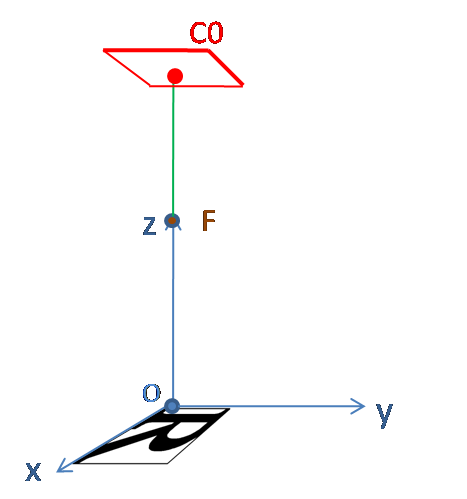
\includegraphics[scale=0.35]{vue_tps_identity.png}}}
		\subfigure[Vue après une première rotation (d'angle $\phi$)]{
		\centering
		{
\includegraphics[scale=0.24]{vue_fps_rotation_phi.png}}
		{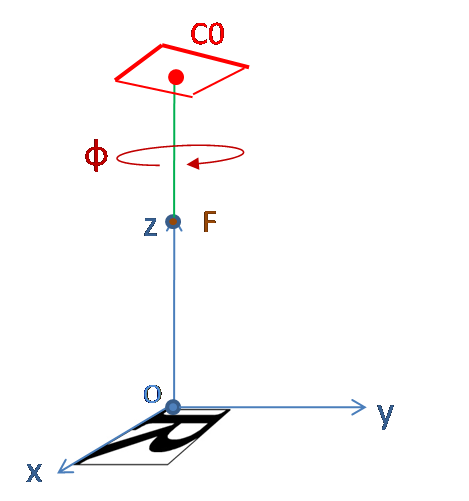
\includegraphics[scale=0.35]{vue_tps_rotation_phi.png}}}
		\subfigure[Vue après l'homographie unidirectionnelle]{
		\centering
		{
\includegraphics[scale=0.24]{vue_fps_hom_part.png}}
		{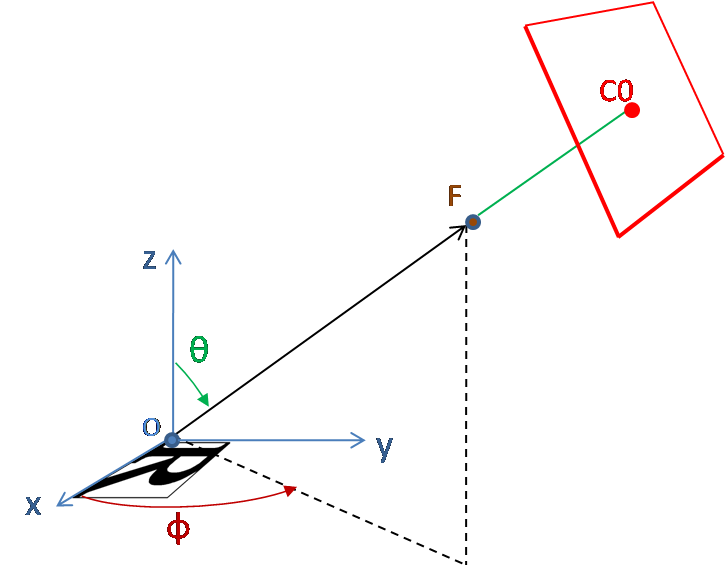
\includegraphics[scale=0.35]{vue_tps_hom_part.png}}}
		\subfigure[Vue finale (après rotation d'angle $\psi$)]{
		\centering
		{
\includegraphics[scale=0.24]{vue_fps_rotation_psi.png}}
		{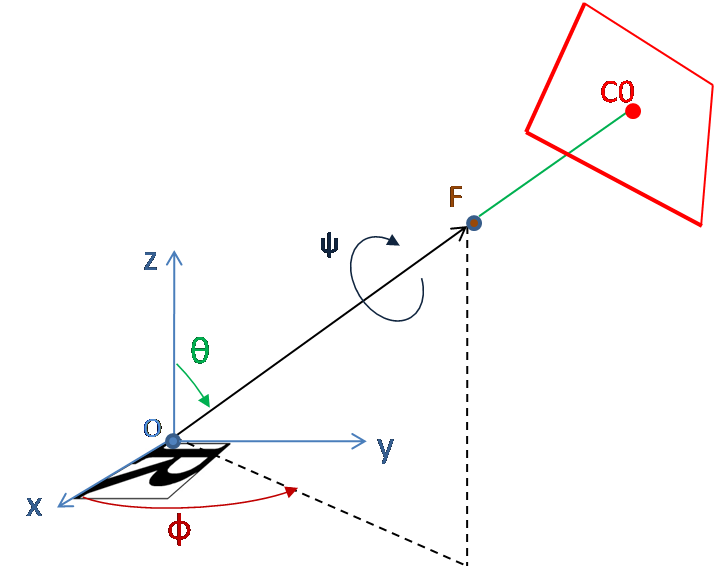
\includegraphics[scale=0.35]{vue_tps_rotation_psi.png}}}
		\caption{Étapes de traitement d'une homographie, assimilées à des mouvements de caméra, à gauche la vue de la caméra, à droite une vue extérieure immobile. Les translations ont été omises pour plus de clarté. Sur les vues extérieures, $F$ représente le point focal de la caméra, le plan rouge est le plan image de la caméra. (cf \ref{ref_schema_decomp_cool})}
		\label{schema_decomp_cool}
		\label{SchemaEtapesDecompoGeometrique}
	\end{figure}
	\clearpage
